\documentclass[12pt, orivec]{article}
\usepackage[no-math]{fontspec}
\usepackage{amsmath}
\usepackage{amssymb}    % for \rightsquigarrow
\usepackage{wasysym}	% for frown face
\usepackage[most]{tcolorbox}
\usepackage{ulem}
\usepackage{tikz-cd}		% commutative diagrams
\usepackage{tikz}
\usepackage{amsthm}
\usepackage{enumitem}	% for \itemize custom labels
\usepackage{turnstile}	% longer turnstiles
\usepackage[sf,bf,big,raggedright,compact]{titlesec}	% change section color to blue
\usepackage[backend=biber,bibstyle=authoryear]{biblatex}
\bibliography{../AGI-book}

\ifdefined\chinchin
	\setromanfont{FreeSans}
	\usepackage[CJKspace]{xeCJK}
	\setCJKmainfont[FallBack, BoldFont=Noto Sans CJK SC Medium, ItalicFont=AR PL KaitiM GB]{Noto Sans CJK SC Light}
	\newcommand{\cc}[2]{#1}
\else
	\setromanfont{Ubuntu}
	\newcommand{\cc}[2]{#2}
\fi

\newtheorem{theorem}{Theorem}

\setcounter{secnumdepth}{0}		% no section numbers

\titleformat{\section}[hang]{\Large\color{blue}}{\thesection \hspace{10pt}}{0pt}{}
\titleformat{\subsection}[hang]{\large\color{blue}}{\thesubsection \hspace{5pt}}{0pt}{}

\newcommand{\book}[1]{$\NewSym[0.4]{../book-icon.png} \quad$ \parbox{0.9\textwidth}{\footnotesize #1}}
\newcommand{\code}[1]{{\footnotesize{\ttfamily #1}}}
\newcommand{\tab}{\hspace*{2cm}}
\newcommand{\powerset}{\raisebox{.15\baselineskip}{\Large\ensuremath{\wp}}}
\newcommand{\Chi}{\raisebox{2.5pt}{$\chi$}}
\newcommand*\KB{\vcenter{\hbox{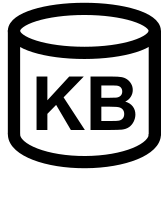
\includegraphics{../KB-symbol.png}}}}
\newcommand*\NewSym[2][0.5]{\vcenter{\hbox{\includegraphics[scale=#1]{#2}}}}
\newcommand*\sigmoid{\vcenter{\hbox{
\includegraphics{sigmoid.png}}}}
\newcommand{\smbox}[1]{\boxed{\footnotesize{\mbox{#1}}}}

\newcommand{\tikzmark}[1]{\tikz[overlay,remember picture] \node (#1) {};}

\newcommand{\Dfrac}[2]{%
	\ooalign{%
		$\genfrac{}{}{2.9pt}0{\hphantom{#1}}{\hphantom{#2}}$\cr%
		$\color{white}\genfrac{}{}{1.5pt}0{\hphantom{#1}}{\hphantom{#2}}$\cr%
		$\color{white}\genfrac{}{}{1pt}0{\color{black}#1}{\color{black}#2}$}}

\renewcommand{\thefootnote}{\fnsymbol{footnote}}
\interfootnotelinepenalty=10000

\title{\color{blue} COCO white paper}
% \author{\cc{甄景贤}{YKY}}

\begin{document}
\setlength{\parindent}{0pt}
\setlength{\parskip}{2.8ex plus0.8ex minus0.8ex}

\maketitle

\begin{abstract}
Coco is a decentralized, autonomous, anonymous, open-source, for-profit, platform for online collaborative projects based on virtual shares.
\end{abstract}

\section{\cc{设计 COCO 的目的}{What does COCO try to solve?}}

\begin{itemize}
	\item \cc{公司的\textbf{股价} 是由外在的自由市场决定(「看不见的手」)}
	{A company's \textbf{stock prices} are determined externally by the free-market (``invisible hand'')}

	\item \cc{公司内部的\textbf{股份},可以由公司自行决定,这是 COCO 企图解决的问题,希望做到比现有方法更好。 }
	{How the company distributes its \textbf{shares} are decided internally;  This is where COCO tries to innovate.}
\end{itemize}

\section{\cc{实名 vs 匿名}{Real-name vs anonymity}}

All contribs are anonymous by default;  Users can use their real names optionally.

\section{Shares}

Contributors get shares automatically when peers vote up their contribs.

When an outside \textbf{investor} puts money into the company, his contrib is treated just like any other contrib.  His investment earns him an amount of shares determined by existing share-holders in the project.  This price may vary depending on the investor's outlook for the project.

\section{Branching}

Branching occurs when there is a dispute whether to include a contrib or not.

After branching, all previous contribs up to that point are included in the new branch.  Then users decide which branch they want to contribute to.



\section{Voting scheme}

Votes (also called ratings) can be any number $\in [-1,1]$.  They represent the \% (percentage shares) a user wants to give to a particular contrib.

All votes are visible for public scrutiny.

If some features (contribs) are seen to be voted unfairly, share-holders may initiate new branches.

\section{Problems}

\begin{itemize}
	\item ``reputation'' may be inaccurate when users have small \# of contribs
	
	\item branching is automatic -- you don't need to care about how others vote, as long as your branch works / someone buys it
	
	\item bad voting should be penalized, but if a contributor is already low-score, the most we can do is to reduce his score to 0.  But since each score is earned either by money or work, the penalty may still make sense.
	
	\item How to prevent the possibility of a significant contributor spawning fake contribs?  But if all the votes are visible, the significant contributor may risk losing his reputation (in the project) even if he is anonymous.  
	
\end{itemize}

其实 自愿 的 voting 和由此建立起的 reputation 有问题,因为 vote 别人不能带来直接的利益,而是一个 management task,传统上由 经理人 做。  但如果要取代这 management 角色,则需要一个相对地完备的机制。   Manager 接受 salary,他的工作是 control tasks, monitor work and give rewards.   问题是这件工作可不可以变成 distributive?  

\section{Buying the product}

Buyers pay for the project's end project, which includes all its branches.

She can choose to deploy any branch for her usage.

By paying for the product, buyers automatically become share-holders.

Buyers have the right to up/down-vote features (contribs) just like other share-holders.

\pagebreak

\section{Potential problems and possible solutions}
\footnotesize

\subsection{\cc{Free-riders 问题}{The problem of free-riders}}

\cc{
按道理,那些不作为的 founders,其股份应该下跌。  但怎样分辨 懒惰的 free-riders 和 要求较高的 founders?
}{
In principle, if a founder hoards shares without performing useful work, his shares in the company should be reduced.	 But how could we distinguish between lazy free-riders and someone who has high standards for other people's work?
}

\cc{
其中一个解决的可能是: 当 founders 们意见不合时可以 \textbf{分叉} (branching),....
}{
A possible solution is via \textbf{branching} when founders disagree with each other.
}

\cc{
分叉的意义是: 保留两种可能。 
}{
The essence of branching is:  to preserve both options in a disagreement.
}

\begin{enumerate}
	\item branch A accepts new contrib X
	\begin{enumerate}
		\item X is a good contrib
		\item X is a bad contrib
	\end{enumerate}
	\item branch B rejects new contrib X
	\begin{enumerate}
		\item X is a good contrib
		\item X is a bad contrib
	\end{enumerate}
\end{enumerate}

\cc{
在 (1b) 和 (2a) 的情况下,branch 1 和 branch 2 分别应该受到惩罚。
}{
In cases (1b) and (2a), branch 1 and 2 should be penalized respectively.
}

\cc{
很明显,应该有 users 能判断哪个是 better branch,但实际上可能出现 branching 太多的问题,还有 users 不能分辨有没有渗入 free-riders 的分支。 
}{
Obviously, there should exist users who can determine which branches are better, but in practice there may be too many branches to consider.  Users may be unable to tell which branches are contaminated with free-riders. 
}

\cc{
但如果所有 votes 是公开的,则在统计上,始终会是较好的 branch 胜出。 
}{
However, if all votes are openly visible, then statistically we may believe that good branches will win out eventually.	
}

\subsection{Insider attacks}

Typical scenario:  a sub-group of insiders systematically up-vote themselves and down-vote outsiders.  They share their identities and contribs among themselves, contrary to COCO's anonymity intention.

Solution:  If some users see their contribs are not voted fairly, they may initiate new branches.

We may have an additional feature to penalize bad voting?

\iffalse

\section{Collective bidding scheme}

Assume that \textbf{initially}, $A, B, ...$ shares the company by the ratio $A : B : ...$.  The new-comer $X$ wants to join.

We use the same symbol $A$ to denote the user as well as the ``value'' (\textbf{equity}) she owns in the company.  

Before bidding, the fraction $\frac{A}{A + B + ...}$ is the \% shares of $A$ in the company $A + B + ...$.

In practice, the equity values \uline{cannot be known internally}, we can only measure their \% percentage shares.  In other words, we always have the normalization
\begin{equation}
A + B + ... = 1
\end{equation}
and the quantities $A, B, ...$ are regarded as percentages.

The actual equity-value of these shares is \textbf{market-determined}.  This is how the traditional stock market works.

\subsection{Scenario 1:  New-comer $X$ offers a contrib and bids (suggests) a share amount}

Each prior member ($A$, $B$, ...) would respond with the \% percentage shares she thinks $X$ may own.  This respond is denoted $\sigma_i \in [0,1] = 0\% ... 100\%$ where $i$ is the \textbf{member index} ($A, B, ... $ etc).

The amount of shares $X$ will get is given by:
\begin{equation}
\label{shares-assigned-to-X}
\frac{X}{A + B + ...} = \sigma_A (\frac{A}{A + B + ...}) + \sigma_B (\frac{B}{A + B + ...}) + ...
\end{equation}
In other words, it is the \textbf{weighted-average} of assigned shares.

Q:  if $A$ \uline{refuses} $X$'s contrib, ie, $\sigma_A = 0$, would $A$'s original shares be \textbf{diluted}?  Under the current scheme, the answer is yes, but the dilution may be reasonable / acceptable.


\subsection{Scenario 2:  Prior member offers a job with a share amount}

In this case, all prior members need to collectively decide if the new-comer has accomplished the task, which is a \textbf{binary} decision (``yes'' or ``no'').


\subsection{After-bidding shares adjustment}

After bidding, prior members' shares must decrease to create $X$'s new shares.

The shares assigned to $X$ is given by (\ref{shares-assigned-to-X}).  So the prior members must split the \textbf{remaining} shares among themselves:
\begin{equation}
\boxed{\mbox{remainder}} \quad r = 1 - X / \mathcal{E}
\end{equation}
where we used the shorthand $\mathcal{E} = A + B + ...$, \textit{ie}, the normalization factor.

Each prior member's shares can be renewed via this formula:
\begin{equation}
A = r \cdot \frac{\sigma_B + \sigma_C + ...}{\sum \sigma_i}
\end{equation}

\section{\cc{一些经济学理论背景}{Some economic-theoretical background}}

\cc{
	一班人合作创造一件 product,这件商品的 \textbf{价格} 是由 \textbf{市场} 决定的。  这个思想可以追溯到 Adam Smith 在 1776 年 提出的 \textbf{自由市场} 理论,亦即是经济学里最基础的理论。 而自由市场这一思想,甚至可以说 符合了 后来 Charles Darwin 在 1859 年 提出的 生物的 \textbf{进化论}。  COCO 假设自由市场的基本条件成立。
}{
	When a group of people creates a \textbf{product}, its \textbf{price} is determined by the \textbf{market}.  This idea, first articulated by Adam Smith in 1776, is one of the foundational principles of all economics.  It can be said that free-market competition is also congruent with the idea of biological \textbf{evolution}, posited by Charles Darwin, later in 1859.  We assume here that the conditions of free-market economics are satisfied.
}

\cc{
	在 1859-60's,Karl Marx 发表了《资本论》,其中提出了 著名的 \textbf{剩馀价值 理论},认为 商品 的价值是投入的 \textbf{资本} 和 \textbf{劳动力} 的某个 \textbf{函数}。  这个假设现在受到很大质疑,因为 价值 和投入的 劳动力 之间,可以有非常复杂而非线性的关系。 
}{
	Around 1859-60's, Karl Marx published \textit{Das Kapital}, in which he posited the now-famous theory of \textbf{surplus values}.  According to this view, the value of a commodity is construed as a function of the input of \textbf{capital} and \textbf{labor}.  Currently, this assumption is thrown into great doubt because the value of a product may depend on input labor in highly complex and non-linear relations.
}

\cc{
	\textbf{股份公司} 的概念是资本主义最伟大的发明之一。  \textbf{公司} (company) 制造 product,product 的价格由外面的市场决定,但合作者在公司内的 \textbf{股份} (shares) 是可以由公司内部决定的。  后者就是 COCO 企图解决的问题,或许可以做到比现有方法更好。
}{
	Economists would agree that the notion of \textbf{joint-stock companies} is one of the greatest inventions of capitalism.  While prices are determined externally by markets, the shares of a company that a participant owns can be decided internally by the company.  The goal of COCO is to provide a (hopefully) better method of distributing shares for online companies.
}

\fi

\printbibliography

\end{document}